\newif\ifglobal

%%%%%%%%%%%%%%%%%%%%%%%
%%% Compile to view %%%
%%%%%%%%%%%%%%%%%%%%%%%

%%%%%%%%%%%%%%%%%%%%%%%%%%%%%%%%%%%%%%%%%%%%%%%%%%%
%%% Readme:                                     %%%
%%% https://www.overleaf.com/read/bwdjvfjksvjy/ %%%
%%%%%%%%%%%%%%%%%%%%%%%%%%%%%%%%%%%%%%%%%%%%%%%%%%%

% >>> M?: marks a module setting number or important notice

% >>> M4: Set {./relative-path} to external files for this module <<<
\def \modulefiles {./27-EXTMEMENCR}
% To add an external file, use:
% (Replace '---' with actual filename)
% '\input{\modulefiles/tables/---.tex}' for tables
% '\includegraphics{\modulefiles/figures/---}' for figures
% '\subfile{\modulefiles/---}' for register files


% >>> M1: This module is in global project? <<<
% 'YES' - uncomment; 'NO' - comment out
\globaltrue

\ifglobal
    \documentclass[main\_\_CN.tex]{subfiles}
   
\else
    % Font "FandolSong-Regular" used by ctex does not have GSUB table.
    % It causes warnings that do not affect compilation and can be ignored.
    \PassOptionsToPackage{quiet}{fontspec}

    \documentclass[openany, 10pt]{book}
   
    % >>> M2: In ./00-shared/preamble-trm-module, also find
    %         settings for visibility of todo notes, watermark <<< 
    \usepackage{preamble-trm-module}


    % Enable Chinese typesetting
    \usepackage{ctex}

    % >>> M3: Temporary labels in Chinese
    %         you can add your own labels there <<<
    \myexternaldocument{./00-shared/temp-labels-cn}

\fi %\ifglobal


\setcounter{secnumdepth}{4}


% >>> M5: If this module needs any updates in
% './00-shared/preamble-trm-module.sty'
% (include additional package, etc.), contact your module PM
% or create the file './00-shared/changelog.tex' make the
% necessary updates yourself and document them in this file <<<


\begin{document}


% Sets language into which pre-defined bits of text are translated
\selectlanguage{chinese}

% Do not delete this block
\ifglobal
% Add the following front matter if
% this module is outside of global project
\else
    \InputIfFileExists{readme}{}{}
    {\let\clearpage\relax \listoftodos}
    \tableofcontents
    %\listoftables
    %\listoffigures
\fi



%%%%%%%%%%%%%%%%%%%%%%%%%
%%% TRM Module Begins %%%
%%%%%%%%%%%%%%%%%%%%%%%%%

\chapter{片外存储器加密与解密 (XTS\_AES)}
\label{mod:extmemencr}
\hypertarget{extmemencr}{}


\section{概述}

\chipname{} 芯片集成了片外存储器加密与解密模块，采用符合 \href{https://ieeexplore.ieee.org/document/4493450}{IEEE Std 1619-2007} 指定的 XTS-AES 标准算法，为用户存放在片外存储器 (flash) 的应用代码和数据提供了安全保障。用户可以将专有固件、敏感的用户数据（如用来访问私有网络的证书）存放在片外 flash 中。


\section{主要特性}

\begin{itemize}
    \item 通用 XTS-AES 算法，符合 IEEE Std 1619-2007
    \item 手动加密过程需要软件参与
    \item 高速的自动解密过程，无需软件参与
    \item 寄存器配置、eFuse 参数、启动 (boot) 模式共同决定加解密功能
\end{itemize}


\section{模块结构}
片外存储器加解密模块包含两个部分：手动加密 (Manual Encryption) 模块和自动解密 (Auto Decryption) 模块。结构图如图 \ref{fig:extmemencr-arch-ext-mem-encr-decr} 所示。


\begin{figure}[H]
    \centering
    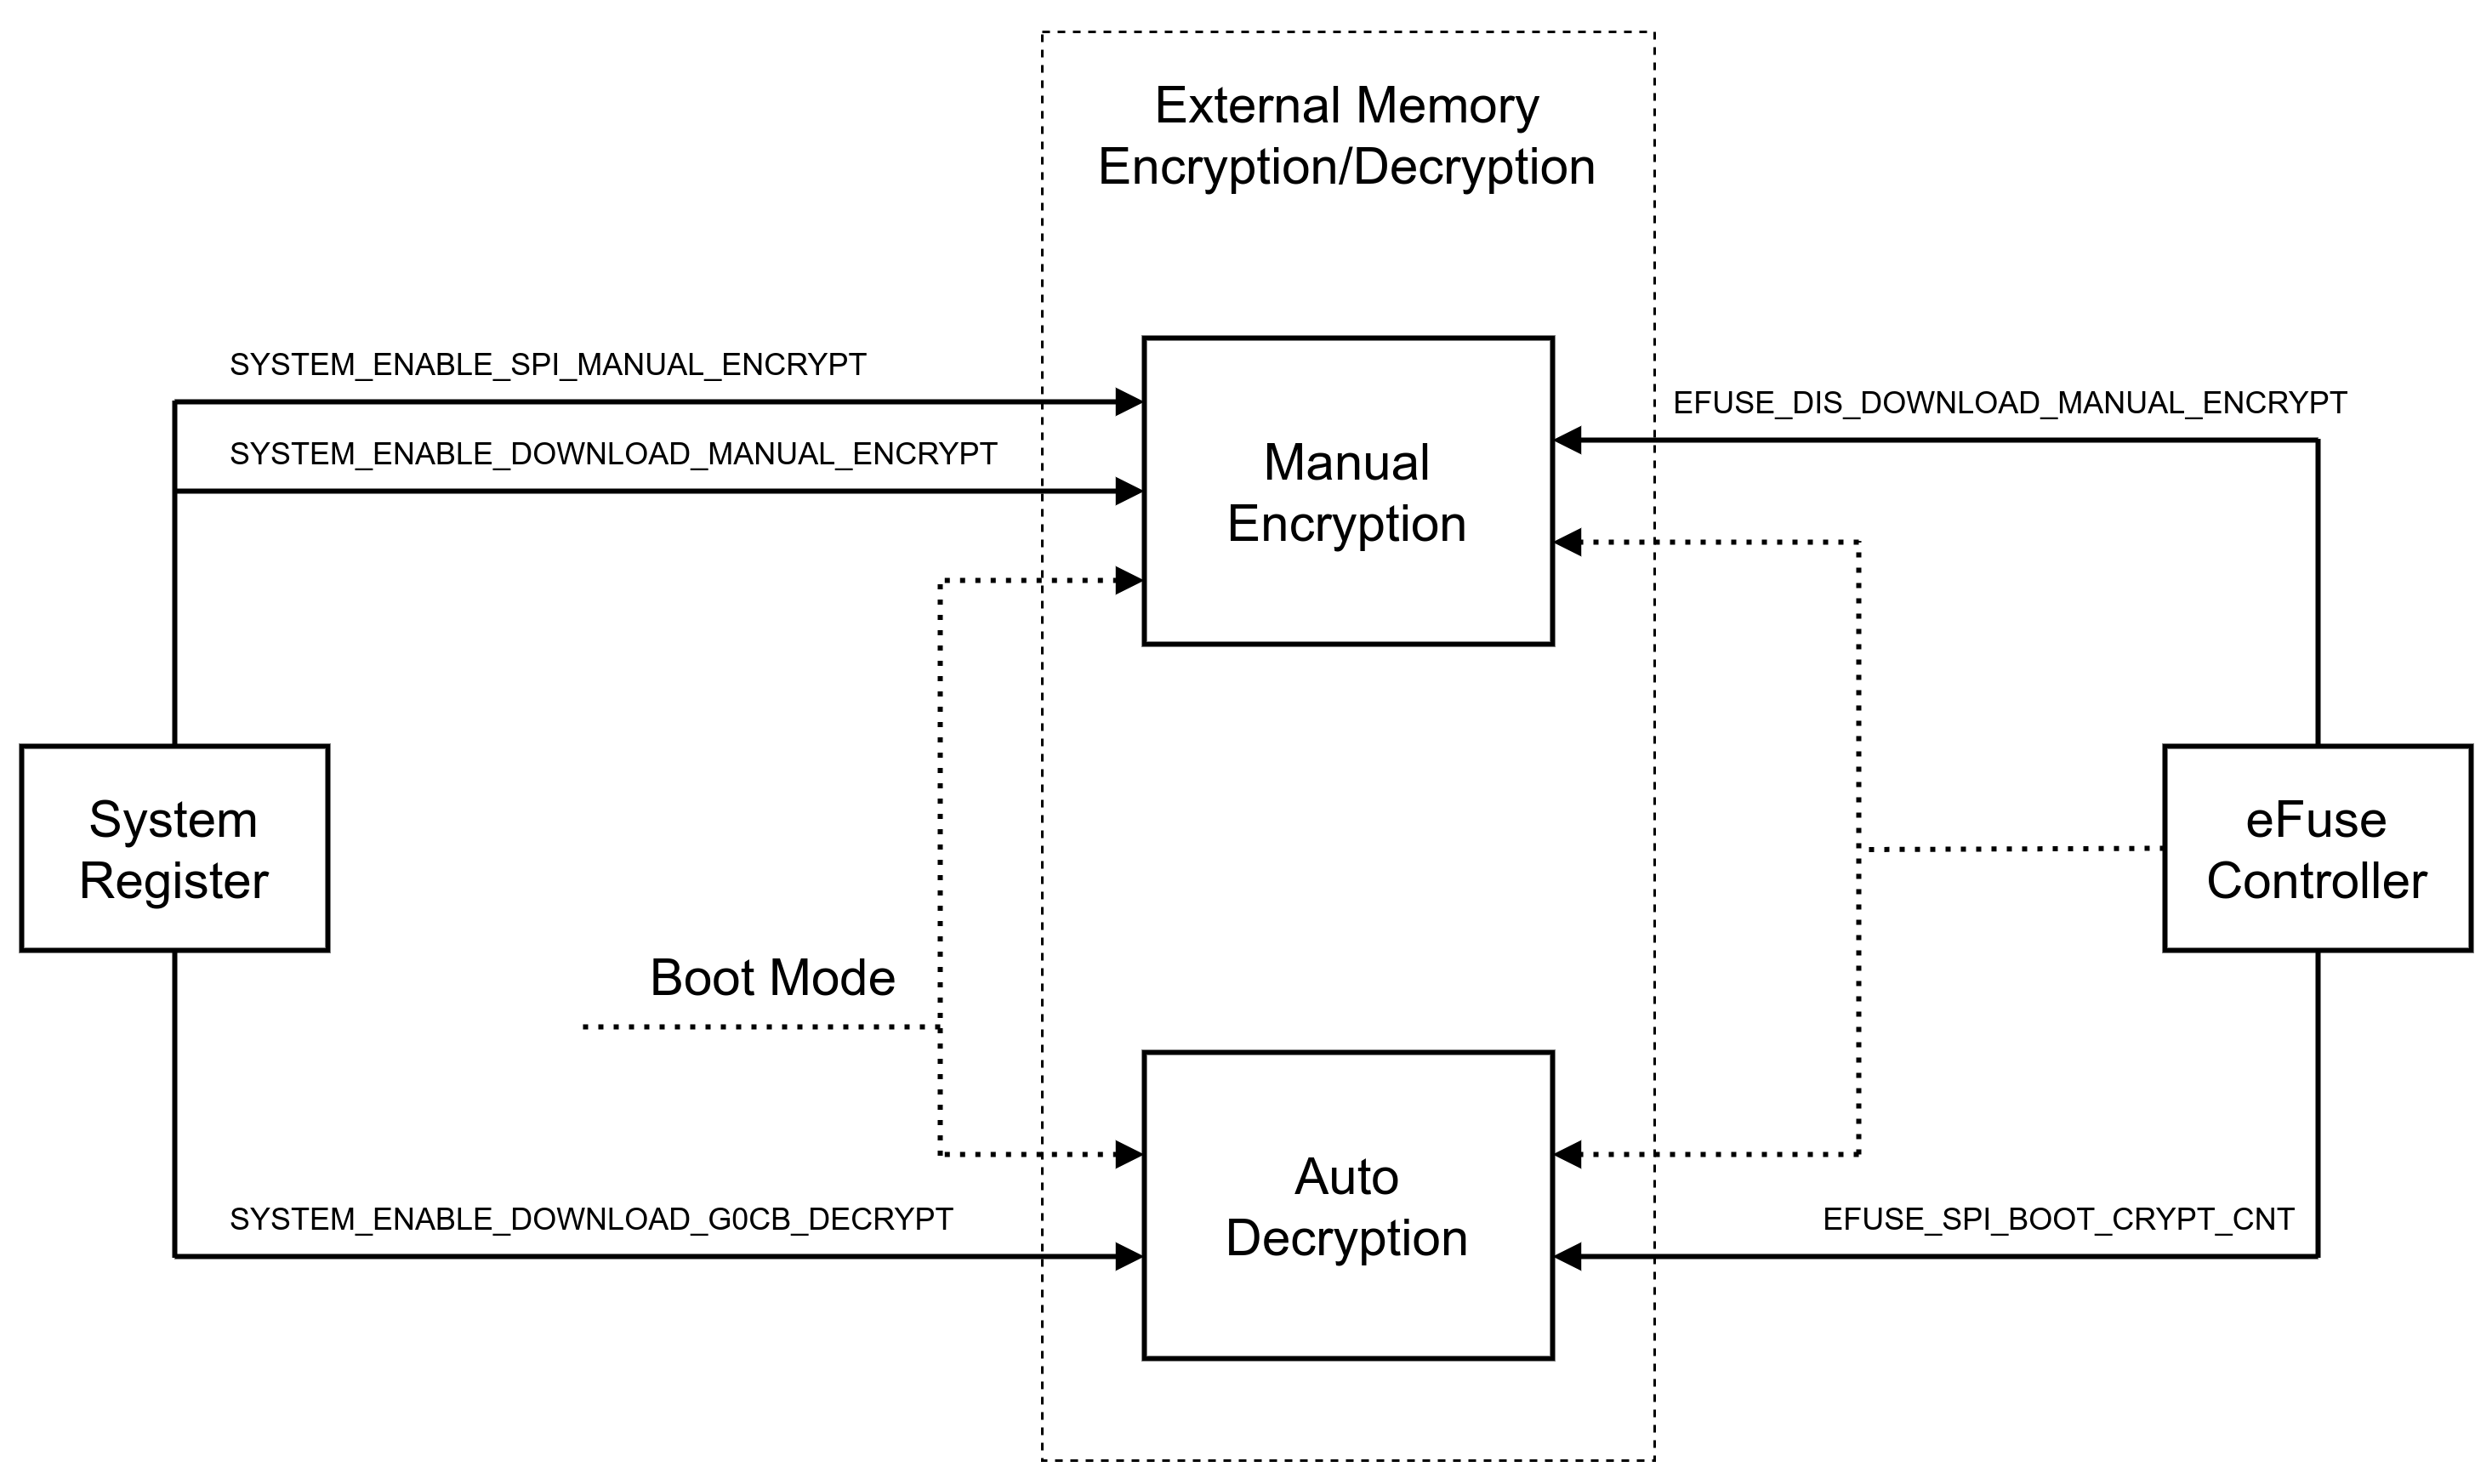
\includegraphics[width=0.8\textwidth]{./27-EXTMEMENCR/figures/27-EXTMEMENCR-external-memory-cryptography}
    \caption{片外存储器加解密结构}
    \label{fig:extmemencr-arch-ext-mem-encr-decr}
\end{figure}

手动加密模块能够对指令/数据进行加密，指令/数据将以密文状态通过 SPI1 被写入片外 flash。

系统寄存器 (SYSREG) 外设中（请参见 \ref{mod:sysreg} \textit{\nameref{mod:sysreg}}）\\ \hyperref[regdesc:SYSTEMEXTERNALDEVICEENCRYPTDECRYPTCONTROLREG]{SYSTEM\_EXTERNAL\_DEVICE\_ENCRYPT\_DECRYPT\_CONTROL\_REG} 内的以下 4 个位与片外存储器加解密相关：
\begin{itemize}
    \item \hyperref[fielddesc:SYSTEMENABLEDOWNLOADMANUALENCRYPT]{SYSTEM\_ENABLE\_DOWNLOAD\_MANUAL\_ENCRYPT} 
    \item \hyperref[fielddesc:SYSTEMENABLEDOWNLOADG0CBDECRYPT]{SYSTEM\_ENABLE\_DOWNLOAD\_G0CB\_DECRYPT} 
    \item \hyperref[fielddesc:SYSTEMENABLEDOWNLOADDBENCRYPT]{SYSTEM\_ENABLE\_DOWNLOAD\_DB\_ENCRYPT} 
    \item \hyperref[fielddesc:SYSTEMENABLESPIMANUALENCRYPT]{SYSTEM\_ENABLE\_SPI\_MANUAL\_ENCRYPT} 
\end{itemize}

片外存储器加解密模块还会从外设 eFuse 控制器中获取 2 个参数：\hyperref[fielddesc:EFUSEDISDOWNLOADMANUALENCRYPT]{EFUSE\_DIS\_DOWNLOAD\_MANUAL\_ENCRYPT} 和 \hyperref[fielddesc:EFUSESPIBOOTCRYPTCNT]{EFUSE\_SPI\_BOOT\_CRYPT\_CNT}。更多详细信息，请参考章节 \ref{mod:efuse} \textit{\nameref{mod:efuse}}。


\section{功能描述}

\subsection{XTS 算法} 
\label{sec:extmemncr-xts-algo}

不论是手动加密，还是自动解密，该模块使用的都是 XTS 算法。
根据算法特征，在具体实现中，使用 1024 位为一个数据单元 (data unit)，此处的“数据单元”由 \textit{XTS-AES Tweakable Block Cipher} 标准中的章节 \textit{XTS-AES encryption procedure} 定义。更多关于 XTS-AES 算法的信息，请参考 \href{https://ieeexplore.ieee.org/document/4493450}{IEEE Std 1619-2007}。

\subsection{密钥} 
\label{sec:extmemncr-key}

在执行 XTS 运算时，手动加密模块和自动解密模块使用完全相同的密钥 \begin{math}Key\end{math} 。密钥 \begin{math}Key\end{math}  来自硬件 eFuse， 且无法被用户访问获取。

密钥 \begin{math}Key\end{math} 的长度为 256 位。\begin{math}Key\end{math} 的值完全由 eFuse 参数信息决定。为方便阐述如何通过 eFuse 参数信息推导出  \begin{math}Key\end{math} 的值，现约定：
\begin{itemize}
    \item Block$_A$：BLOCK4 \verb+~+ BLOCK9 中的密钥用途为 EFUSE\_KEY\_PURPOSE\_XTS\_AES\_128\_KEY 的 BLOCK（请参考表 \ref{tab:efuse-key-purpose} \textit{\nameref{tab:efuse-key-purpose}}）。如果 Block$_A$ 存在，那么 Block$_A$ 中存放着 256 位的 \begin{math}Key_{A}\end{math}。
\end{itemize}

根据 Block$_A$ 是否存在可以产生两种可能性。不同情况下， \begin{math}Key\end{math} 值可以由 \begin{math}Key_{A}\end{math} 的值唯一确定，如表 \ref{tab:extmemencr-key-possibility} 所示。

\begin{longtable}[c]{ |c|c|c|c|c| }
\caption{根据 \begin{math}Key_{A}\end{math} 生成的 \begin{math}Key\end{math} 值}
\label{tab:extmemencr-key-possibility}
\\\hline 
\rowcolor{lightgray}
Block$_A$ 是否存在& \begin{math}Key\end{math}  & \begin{math}Key\end{math} 长度（位） \\\hline
\endfirsthead
\hline
\rowcolor{lightgray}
Block$_A$ 是否存在& \begin{math}Key\end{math}  & \begin{math}Key\end{math} Length (bit) \\\hline
\endhead
\endfoot
是       &   \begin{math}           Key_{A}\end{math}    &   256   \\\hline
否        &   \begin{math}           0^{256}\end{math}    &   256   \\\hline
\end{longtable}
\vspace{-1.5em}
{\bfseries 说明：}\\
表 \ref{tab:extmemencr-key-possibility} 中，``\begin{math}0^{256}\end{math}" 表示由 256 个位 0 组成的位串。


更多有关密钥用途的信息，请参考章节 \ref{mod:efuse} \textit{\nameref{mod:efuse}} 中的表 \ref{tab:efuse-key-purpose} \textit{\nameref{tab:efuse-key-purpose}}。

\subsection{目标空间} 
\label{sec:extmemencr-target-space}

目标空间指：片外存储器 (flash) 中存放首次加密密文的一段连续地址空间。目标空间可由目标大小和目标基地址这两个参数唯一确定。这两个参数的定义如下：

\begin{itemize}
    \item 目标大小：目标空间的大小 (\begin{math} size \end{math})， 以字节为单位，即单次对多少数据进行加密。仅支持 16 和 32 字节。
    \item 目标基地址：目标空间的基地址 (\begin{math} base\_addr\end{math})，这是一个 24 位的物理地址，取值范围为 0x0000\_0000 \verb+~+ 0x00FF\_FFFF， 但要求以 \begin{math} size \end{math} 为单位对齐，即 \begin{math} base\_addr \% size == 0 \end{math}。
\end{itemize}

如某一次加密操作，要将 16 字节的指令数据加密后存放在片外 flash 中的地址段 0x130 \verb+~+ 0x13F 中，则目标空间为 0x130 \verb+~+ 0x13F，目标大小为 16 (字节)，目标基地址为 0x130。

对于任意长度（必须是 16 字节 的整数倍）的明文指令/数据的加密，可以将整个加密过程拆分成多次进行，每次都有各自的目标空间和相应参数。

对于自动解密模块，目标空间等参数由硬件自动调节。对于手动加密模块，目标空间等参数需要用户主动配置。

\begin{tiplisting}
\vspace{-2em}
\begin{enumerate}
     \href{https://ieeexplore.ieee.org/document/4493450}{IEEE Std 1619-2007} 中的章节 \textit{Data units and tweaks} 中定义的 “tweak”  是一个 128-bit 的非负整数（ \begin{math} tweak \end{math}），
    其值可以通过公式求出： \begin{math} tweak \end{math} = (\begin{math} base\_addr \end{math} \& 0x00FFFF80)。\begin{math} tweak \end{math} 中低 7 位和高 97 位恒为零。
\end{enumerate}
\end{tiplisting}

\subsection{数据写入} 
\label{sec:extmemncr-data-writing}

对于自动解密模块，数据的写入由硬件自动完成。对于手动加密模块，数据的写入需要用户主动配置。手动加密模块中包含 8 个寄存器 XTS\_AES\_PLAIN\_\textcolor{red}{\it{n}}\_REG (\textcolor{red}{\it{n}}: 0 \verb+~+ 7) 构成的寄存器块，专用于数据写入，一次可以存放最多 256 位明文指令/数据。

实际上，手动加密模块不在乎明文来自什么地方，只注重密文将要存放在什么地方。考虑到明文和密文之间呈严格的对应关系，为了更好地描述明文如何存放在寄存器块中，现假设明文从一开始就放在目标空间中，并在加密完成后被密文替换。因此，接下来的描述不再出现“明文”这个概念，而用“目标空间”来代替。但请注意，在真正使用时，明文可以来自任何地方，但用户必须清晰知道明文如何存放在寄存器块中。

{\bfseries 目标空间映射到寄存器块的方法：}

假设目标空间中某个字的存放地址为 \begin{math} address \end{math} ，记  \begin{math} offset = address \% 32 \end{math} ，
    \textcolor{red}{\it{$n$}} =  \begin{math} \frac{offset}{4} \end{math} ， 那么该字将被存放在寄存器 XTS\_AES\_PLAIN\_\textcolor{red}{\it{$n$}}\_REG 中。

例如，当目标大小为 32 时，寄存器块中的所有寄存器都将被使用，目标空间中的地址与寄存器块之间的映射关系如表 \ref{tab:extmemencr-data-padding} 所示。

\begin{longtable}[c]
{ |c|p{4.5cm} |c|p{4.5cm}|}
\caption{目标空间与寄存器堆的映射关系} 
\label{tab:extmemencr-data-padding}\\
\hline 
\rowcolor{lightgray}
\begin{math} offset \end{math}&  寄存器  & \begin{math} offset \end{math} &  寄存器 \\\hline
\endfirsthead
\hline
\rowcolor{lightgray}
\begin{math} offset \end{math} &  寄存器  & \begin{math} offset \end{math} &  寄存器   \\\hline
\endhead
\endfoot
0x00 & \hyperref[regdesc:XTSAESPLAINNREG]{XTS\_AES\_PLAIN\_0\_REG} & 0x10 & \hyperref[regdesc:XTSAESPLAINNREG]{XTS\_AES\_PLAIN\_4\_REG} \\\hline 
0x04 & \hyperref[regdesc:XTSAESPLAINNREG]{XTS\_AES\_PLAIN\_1\_REG} & 0x14 & \hyperref[regdesc:XTSAESPLAINNREG]{XTS\_AES\_PLAIN\_5\_REG} \\\hline 
0x08 & \hyperref[regdesc:XTSAESPLAINNREG]{XTS\_AES\_PLAIN\_2\_REG} & 0x18 & \hyperref[regdesc:XTSAESPLAINNREG]{XTS\_AES\_PLAIN\_6\_REG} \\\hline 
0x0C & \hyperref[regdesc:XTSAESPLAINNREG]{XTS\_AES\_PLAIN\_3\_REG} & 0x1C & \hyperref[regdesc:XTSAESPLAINNREG]{XTS\_AES\_PLAIN\_7\_REG} \\\hline 
\end{longtable}


\subsection{手动加密模块}

手动加密模块是一个外设模块，自身带有寄存器，可以被 CPU 直接访问。模块内的寄存器、系统寄存器 (SYSREG) 外设、eFuse 参数、 boot 模式共同配置并使用这一模块。请注意，手动加密模块只能加密片外 flash。

\textbf{ 当且仅当手动加密模块拥有工作权限时，才允许手动加密。}  手动加密模块是否拥有工作权限取决于：

\begin{itemize}

    \item SPI Boot 模式下
    
    当寄存器 \hyperref[regdesc:SYSTEMEXTERNALDEVICEENCRYPTDECRYPTCONTROLREG]{SYSTEM\_EXTERNAL\_DEVICE\_ENCRYPT\_DECRYPT\_CONTROL\_REG} 的 \\ \hyperref[fielddesc:SYSTEMENABLESPIMANUALENCRYPT]{SYSTEM\_ENABLE\_SPI\_MANUAL\_ENCRYPT} 位为 1 时，手动加密模块拥有工作权限，否则无法工作。
    
    \item Download Boot 模式下
    
    当寄存器 \hyperref[regdesc:SYSTEMEXTERNALDEVICEENCRYPTDECRYPTCONTROLREG]{SYSTEM\_EXTERNAL\_DEVICE\_ENCRYPT\_DECRYPT\_CONTROL\_REG} 的\\ \hyperref[fielddesc:SYSTEMENABLEDOWNLOADMANUALENCRYPT]{SYSTEM\_ENABLE\_DOWNLOAD\_MANUAL\_ENCRYPT} 位为 1，且 eFuse 参数\\ \hyperref[fielddesc:EFUSEDISDOWNLOADMANUALENCRYPT]{EFUSE\_DIS\_DOWNLOAD\_MANUAL\_ENCRYPT} 为 0 时，
    手动加密模块拥有工作权限，否则无法工作。
    
\end{itemize}

\begin{tiplisting}
\vspace{-2em}
\begin{itemize}
\item 即使 CPU 可以越过 cache，直接读片外存储器从而得到加密指令/数据，
但用户还是绝对无法获取到密钥 \begin{math}Key\end{math}。
\end{itemize}
\end{tiplisting}


\subsection{自动解密模块}

自动解密并非传统外设模块，自身不带寄存器，不能被 CPU 直接访问。系统寄存器 (SYSREG) 外设、eFuse 参数、boot 模式共同配置并使用这一模块。

\textbf{当且仅当自动解密模块拥有工作权限时，才允许自动解密。}自动解密模块是否拥有工作权限取决于：

\begin{itemize}
    
    \item SPI Boot 模式下
    
    当参数 SPI\_BOOT\_CRYPT\_CNT（3 位）中奇数个位为 1 时，自动解密模块拥有工作权限，否则无法工作。
    
    \item Download Boot 模式下
    
    当寄存器 \hyperref[regdesc:SYSTEMEXTERNALDEVICEENCRYPTDECRYPTCONTROLREG]{SYSTEM\_EXTERNAL\_DEVICE\_ENCRYPT\_DECRYPT\_CONTROL\_REG} 的 \\ \hyperref[fielddesc:SYSTEMENABLEDOWNLOADG0CBDECRYPT]{SYSTEM\_ENABLE\_DOWNLOAD\_G0CB\_DECRYPT} 位为 1 时，自动解密模块拥有工作权限，否则无法工作。
    
\end{itemize}


\begin{tiplisting}
\vspace{-2em}
\begin{itemize}

\item 当自动解密模块拥有工作权限时，如果 CPU 通过 cache 读取片外存储器中的指令/数据，自动解密将自动对读取到的密文进行解密以恢复指令/数据。解密的整个过程无需软件参与并且对 cache 是透明的。解密算法过程中密钥 \begin{math}Key\end{math} 绝对无法被用户获取。

\item 当自动解密模块没有工作权限时，自动解密模块不对片外存储器中的数据产生作用，无论是加密内容还是未加密内容，因此 CPU 通过 cache 读取到的是片外存储器中的原始内容。

\end{itemize}
\end{tiplisting}


\section{ 软件流程 }
手动加密模块工作时需要软件参与，软件流程为：

\begin{enumerate}
    
    \item 配置 XTS\_AES： 
    \begin{itemize}
        \item 将寄存器 \hyperref[regdesc:XTSAESPHYSICALADDRESSREG]{XTS\_AES\_PHYSICAL\_ADDRESS\_REG} 的值设置为 \begin{math}base\_addr\end{math}。
        \item 将寄存器 \hyperref[regdesc:XTSAESLINESIZEREG]{XTS\_AES\_LINESIZE\_REG} 的值设置为 \begin{math}\frac{size}{32}\end{math}。
    \end{itemize}
    关于 \begin{math} base\_addr\end{math} 和 \begin{math}size\end{math} 的定义，请参考章节 \ref{sec:extmemencr-target-space}。
    \item 将明文数据写入至寄存器块 XTS\_AES\_PLAIN\_\textcolor{red}{\it{n}}\_REG (\textcolor{red}{\it{n}}: 0 \verb+~+ 7)。更多详细信息，请参考章节 \ref{sec:extmemncr-data-writing}。\\请根据您的实际需求写入寄存器，未使用的寄存器可为任意值。
    
    \item 等待手动加密模块成为空闲状态。轮询寄存器 \hyperref[regdesc:XTSAESSTATEREG]{XTS\_AES\_STATE\_REG} 直到软件读取到 0。
    
    \item 向寄存器 \hyperref[regdesc:XTSAESTRIGGERREG]{XTS\_AES\_TRIGGER\_REG} 写入 1，启动手动加密。
    
    \item 等待加密完成。轮询寄存器 \hyperref[regdesc:XTSAESSTATEREG]{XTS\_AES\_STATE\_REG}，直到软件读取到 2。\\
    上述步骤为使用 \begin{math}Key\end{math} 操作手动加密模块对明文指令进行加密的过程。
    
    \item 向寄存器 \hyperref[regdesc:XTSAESRELEASEREG]{XTS\_AES\_RELEASE\_REG} 写入 1，使 SPI1 获得密文的访问权限。然后，寄存器 \hyperref[regdesc:XTSAESSTATEREG]{XTS\_AES\_STATE\_REG} 的值将为 3。
    
    \item 调用 SPI1，将密文写入片外 flash（请参阅章节 \ref{mod:spi} \textit{\nameref{mod:spi}}）。
    
    \item 向寄存器 \hyperref[regdesc:XTSAESDESTROYREG]{XTS\_AES\_DESTROY\_REG} 写入 1，销毁密文。然后，寄存器 \hyperref[regdesc:XTSAESSTATEREG]{XTS\_AES\_STATE\_REG} 的值将为 0。
    
\end{enumerate}

重复上述步骤，即可满足明文指令/数据的加密需求。


% >>> If your module has no registers, delete sample text
%       for Sections Register Summary and Registers below <<<

%%%%%%%%%%%%%%%%%%%%%%%%
%%% Register Summary %%%
%%%%%%%%%%%%%%%%%%%%%%%%

% >>> Update the sample text below and insert
%     the info on register summary into the subfile <<<

\clearpage
\section{寄存器列表}
\label{sec:extmemencr-reg-summ}
\hypertarget{extmemencr-reg-summ}{}

本小节的所有地址均为相对于片外存储器加密与解密基地址的地址偏移量（相对地址），具体基地址请见章节 \ref{mod:sysmem} \textit{\nameref{mod:sysmem}} 中的表 \ref{tab:sysmem-base-address}。

请查看章节 \hyperref[glossary-access-types]{\textit{寄存器的访问类型}}，了解“访问”列缩写的含义。

\subfile{\modulefiles/27-EXTMEMENCR-reg-summ__CN}


%%%%%%%%%%%%%%%%%
%%% Registers %%%
%%%%%%%%%%%%%%%%%

% >>> Update the sample text below and insert
%      the info on registers into the subfile <<<

\clearpage
\section{寄存器}

本小节的所有地址均为相对片外存储器加密与解密基地址的地址偏移量（相对地址），具体基地址请见章节 \ref{mod:sysmem} \textit{\nameref{mod:sysmem}} 中的表 \ref{tab:sysmem-base-address}。

\subfile{\modulefiles/27-EXTMEMENCR-reg__CN}


\end{document}
